\documentclass[tikz,border=12pt]{standalone}
\usepackage[T1]{fontenc}
\usepackage{lmodern,amsmath}
\usetikzlibrary{arrows.meta}
\definecolor{ink}{HTML}{183444}
\definecolor{blue}{HTML}{1B6780}
\definecolor{amber}{HTML}{AD601A}
\begin{document}
\hyphenpenalty=10000\exhyphenpenalty=10000
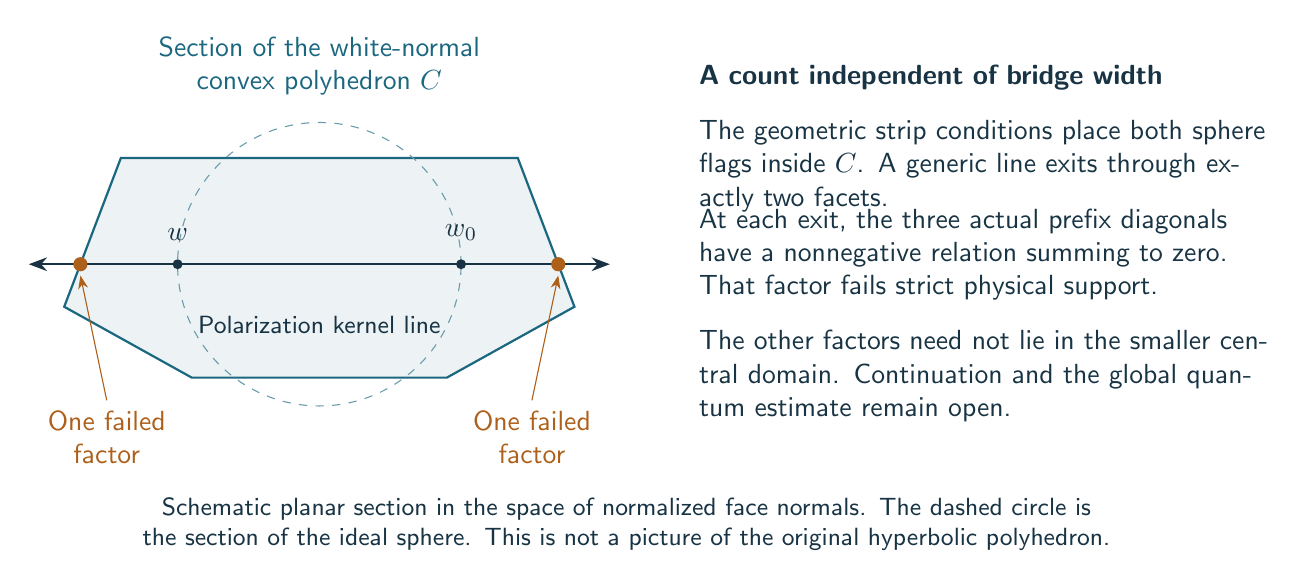
\begin{tikzpicture}[font=\sffamily,text=ink,>=Stealth]
 \begin{scope}[scale=1.8]
  \fill[blue!8] (-1.8,-.3)--(-.9,-.8)--(.9,-.8)--(1.8,-.3)--(1.4,.75)--(-1.4,.75)--cycle;
  \draw[blue,thick] (-1.8,-.3)--(-.9,-.8)--(.9,-.8)--(1.8,-.3)--(1.4,.75)--(-1.4,.75)--cycle;
  \draw[blue!65,dashed] (0,0) circle (1);
  \draw[ink,thick,<->] (-2.05,0)--(2.05,0);
  \foreach \x/\label in {-1/{w},1/{w_0}} {
   \fill[ink] (\x,0) circle (.035);
   \node[above=5pt] at (\x,0) {$\label$};
  }
  \foreach \x in {-1.6857,1.6857} {
   \fill[amber] (\x,0) circle (.05);
  }
  \node[amber,align=center] at (-1.5,-1.22) {One failed\\factor};
  \node[amber,align=center] at (1.5,-1.22) {One failed\\factor};
  \draw[amber,->] (-1.5,-.96)--(-1.6857,-.08);
  \draw[amber,->] (1.5,-.96)--(1.6857,-.08);
  \node[blue,align=center] at (0,1.4) {Section of the white-normal\\convex polyhedron $C$};
  \node[align=center,font=\sffamily\small] at (0,-.43) {Polarization kernel line};
 \end{scope}
 \node[anchor=west,align=left,text width=7.3cm] at (4.7,1.6) {
  \textbf{A count independent of bridge width}\\[8pt]
  The geometric strip conditions place both sphere flags inside $C$.
  A generic line exits through exactly two facets.};
 \node[anchor=west,align=left,text width=7.3cm] at (4.7,-.65) {
  At each exit, the three actual prefix diagonals have a nonnegative
  relation summing to zero. That factor fails strict physical support.\\[8pt]
  The other factors need not lie in the smaller central domain.
  Continuation and the global quantum estimate remain open.};
 \node[align=center,font=\sffamily\small,text width=14.5cm] at (3.9,-3.3) {
  Schematic planar section in the space of normalized face normals.
  The dashed circle is the section of the ideal sphere.
  This is not a picture of the original hyperbolic polyhedron.};
\end{tikzpicture}
\end{document}
